\chapter*{Deliberate discovery}

\ifnotes
    Learning outcomes:
    
    \begin{itemize}
        \item Explain how communication is a major source of defects
        \item Give examples of how requirements are never well understood at the beginning of a project
        \item Describe how these problems have existed forever and that 'agile' on its own cannot solve it
    \end{itemize}
    
    When reviewing the Deliberate Discovery concept, I usually tie this BDD back to money. I ask "why are you paying for BDD training?" and keeping asking "why?" until we get to cost savings. 
    
    I'll often draw a cost vs time exponential graph and tell the 10x story "it's ten time cheaper to fix a defect during development than in test... etc."
    
    I'll stress that "doing testing earlier" encompasses the Liz Keogh quotes about "learning being the constraint", so focus on learning early.
\fi

\ifcontent
    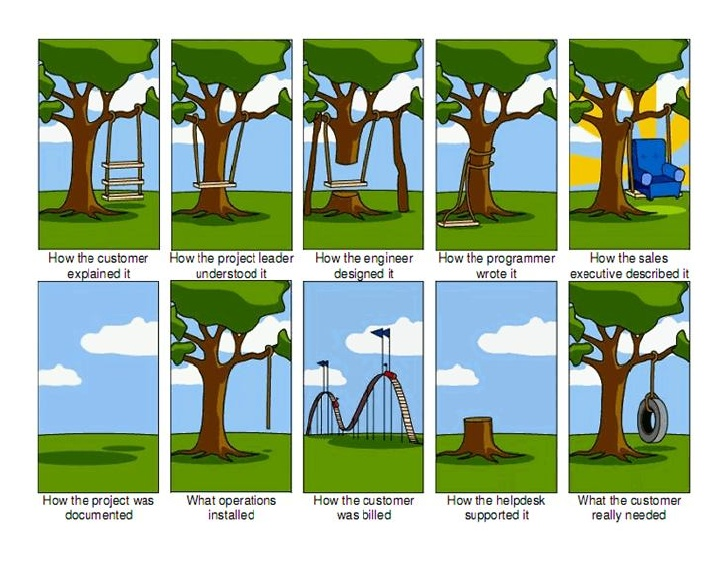
\includegraphics[width=0.9\textwidth, keepaspectratio]{images/project-cartoon}
    
    % We can't use \QandAbox{} on this page, because the embedded \minipage screws up the \footnote
    
    What do you recognise, in this cartoon\footnote{http://projectcartoon.org}, that is similar to projects you've worked on?
    
    \answerbox{1}
    
    What do you think are the main reasons software projects go wrong?
    
    \answerbox{1}
    
    Think about a project you worked on that went well. What was different?
    
    \answerbox{1}
\fi